% Options for packages loaded elsewhere
\PassOptionsToPackage{unicode}{hyperref}
\PassOptionsToPackage{hyphens}{url}
%
\documentclass[
]{book}
\title{R pour l'économétrie}
\author{Abdoul Oudouss Diakite}
\date{}

\usepackage{amsmath,amssymb}
\usepackage{lmodern}
\usepackage{iftex}
\ifPDFTeX
  \usepackage[T1]{fontenc}
  \usepackage[utf8]{inputenc}
  \usepackage{textcomp} % provide euro and other symbols
\else % if luatex or xetex
  \usepackage{unicode-math}
  \defaultfontfeatures{Scale=MatchLowercase}
  \defaultfontfeatures[\rmfamily]{Ligatures=TeX,Scale=1}
\fi
% Use upquote if available, for straight quotes in verbatim environments
\IfFileExists{upquote.sty}{\usepackage{upquote}}{}
\IfFileExists{microtype.sty}{% use microtype if available
  \usepackage[]{microtype}
  \UseMicrotypeSet[protrusion]{basicmath} % disable protrusion for tt fonts
}{}
\makeatletter
\@ifundefined{KOMAClassName}{% if non-KOMA class
  \IfFileExists{parskip.sty}{%
    \usepackage{parskip}
  }{% else
    \setlength{\parindent}{0pt}
    \setlength{\parskip}{6pt plus 2pt minus 1pt}}
}{% if KOMA class
  \KOMAoptions{parskip=half}}
\makeatother
\usepackage{xcolor}
\IfFileExists{xurl.sty}{\usepackage{xurl}}{} % add URL line breaks if available
\IfFileExists{bookmark.sty}{\usepackage{bookmark}}{\usepackage{hyperref}}
\hypersetup{
  pdftitle={R pour l'économétrie},
  pdfauthor={Abdoul Oudouss Diakite},
  hidelinks,
  pdfcreator={LaTeX via pandoc}}
\urlstyle{same} % disable monospaced font for URLs
\usepackage{color}
\usepackage{fancyvrb}
\newcommand{\VerbBar}{|}
\newcommand{\VERB}{\Verb[commandchars=\\\{\}]}
\DefineVerbatimEnvironment{Highlighting}{Verbatim}{commandchars=\\\{\}}
% Add ',fontsize=\small' for more characters per line
\usepackage{framed}
\definecolor{shadecolor}{RGB}{248,248,248}
\newenvironment{Shaded}{\begin{snugshade}}{\end{snugshade}}
\newcommand{\AlertTok}[1]{\textcolor[rgb]{0.94,0.16,0.16}{#1}}
\newcommand{\AnnotationTok}[1]{\textcolor[rgb]{0.56,0.35,0.01}{\textbf{\textit{#1}}}}
\newcommand{\AttributeTok}[1]{\textcolor[rgb]{0.77,0.63,0.00}{#1}}
\newcommand{\BaseNTok}[1]{\textcolor[rgb]{0.00,0.00,0.81}{#1}}
\newcommand{\BuiltInTok}[1]{#1}
\newcommand{\CharTok}[1]{\textcolor[rgb]{0.31,0.60,0.02}{#1}}
\newcommand{\CommentTok}[1]{\textcolor[rgb]{0.56,0.35,0.01}{\textit{#1}}}
\newcommand{\CommentVarTok}[1]{\textcolor[rgb]{0.56,0.35,0.01}{\textbf{\textit{#1}}}}
\newcommand{\ConstantTok}[1]{\textcolor[rgb]{0.00,0.00,0.00}{#1}}
\newcommand{\ControlFlowTok}[1]{\textcolor[rgb]{0.13,0.29,0.53}{\textbf{#1}}}
\newcommand{\DataTypeTok}[1]{\textcolor[rgb]{0.13,0.29,0.53}{#1}}
\newcommand{\DecValTok}[1]{\textcolor[rgb]{0.00,0.00,0.81}{#1}}
\newcommand{\DocumentationTok}[1]{\textcolor[rgb]{0.56,0.35,0.01}{\textbf{\textit{#1}}}}
\newcommand{\ErrorTok}[1]{\textcolor[rgb]{0.64,0.00,0.00}{\textbf{#1}}}
\newcommand{\ExtensionTok}[1]{#1}
\newcommand{\FloatTok}[1]{\textcolor[rgb]{0.00,0.00,0.81}{#1}}
\newcommand{\FunctionTok}[1]{\textcolor[rgb]{0.00,0.00,0.00}{#1}}
\newcommand{\ImportTok}[1]{#1}
\newcommand{\InformationTok}[1]{\textcolor[rgb]{0.56,0.35,0.01}{\textbf{\textit{#1}}}}
\newcommand{\KeywordTok}[1]{\textcolor[rgb]{0.13,0.29,0.53}{\textbf{#1}}}
\newcommand{\NormalTok}[1]{#1}
\newcommand{\OperatorTok}[1]{\textcolor[rgb]{0.81,0.36,0.00}{\textbf{#1}}}
\newcommand{\OtherTok}[1]{\textcolor[rgb]{0.56,0.35,0.01}{#1}}
\newcommand{\PreprocessorTok}[1]{\textcolor[rgb]{0.56,0.35,0.01}{\textit{#1}}}
\newcommand{\RegionMarkerTok}[1]{#1}
\newcommand{\SpecialCharTok}[1]{\textcolor[rgb]{0.00,0.00,0.00}{#1}}
\newcommand{\SpecialStringTok}[1]{\textcolor[rgb]{0.31,0.60,0.02}{#1}}
\newcommand{\StringTok}[1]{\textcolor[rgb]{0.31,0.60,0.02}{#1}}
\newcommand{\VariableTok}[1]{\textcolor[rgb]{0.00,0.00,0.00}{#1}}
\newcommand{\VerbatimStringTok}[1]{\textcolor[rgb]{0.31,0.60,0.02}{#1}}
\newcommand{\WarningTok}[1]{\textcolor[rgb]{0.56,0.35,0.01}{\textbf{\textit{#1}}}}
\usepackage{longtable,booktabs,array}
\usepackage{calc} % for calculating minipage widths
% Correct order of tables after \paragraph or \subparagraph
\usepackage{etoolbox}
\makeatletter
\patchcmd\longtable{\par}{\if@noskipsec\mbox{}\fi\par}{}{}
\makeatother
% Allow footnotes in longtable head/foot
\IfFileExists{footnotehyper.sty}{\usepackage{footnotehyper}}{\usepackage{footnote}}
\makesavenoteenv{longtable}
\usepackage{graphicx}
\makeatletter
\def\maxwidth{\ifdim\Gin@nat@width>\linewidth\linewidth\else\Gin@nat@width\fi}
\def\maxheight{\ifdim\Gin@nat@height>\textheight\textheight\else\Gin@nat@height\fi}
\makeatother
% Scale images if necessary, so that they will not overflow the page
% margins by default, and it is still possible to overwrite the defaults
% using explicit options in \includegraphics[width, height, ...]{}
\setkeys{Gin}{width=\maxwidth,height=\maxheight,keepaspectratio}
% Set default figure placement to htbp
\makeatletter
\def\fps@figure{htbp}
\makeatother
\setlength{\emergencystretch}{3em} % prevent overfull lines
\providecommand{\tightlist}{%
  \setlength{\itemsep}{0pt}\setlength{\parskip}{0pt}}
\setcounter{secnumdepth}{5}
\usepackage{booktabs}
\ifLuaTeX
  \usepackage{selnolig}  % disable illegal ligatures
\fi
\usepackage[]{natbib}
\bibliographystyle{apalike}

\usepackage{amsthm}
\newtheorem{theorem}{Theorem}[chapter]
\newtheorem{lemma}{Lemma}[chapter]
\newtheorem{corollary}{Corollary}[chapter]
\newtheorem{proposition}{Proposition}[chapter]
\newtheorem{conjecture}{Conjecture}[chapter]
\theoremstyle{definition}
\newtheorem{definition}{Definition}[chapter]
\theoremstyle{definition}
\newtheorem{example}{Example}[chapter]
\theoremstyle{definition}
\newtheorem{exercise}{Exercise}[chapter]
\theoremstyle{definition}
\newtheorem{hypothesis}{Hypothesis}[chapter]
\theoremstyle{remark}
\newtheorem*{remark}{Remark}
\newtheorem*{solution}{Solution}
\begin{document}
\maketitle

{
\setcounter{tocdepth}{1}
\tableofcontents
}
\hypertarget{bienvenue}{%
\chapter*{Bienvenue}\label{bienvenue}}
\addcontentsline{toc}{chapter}{Bienvenue}

This is a \emph{sample} book written in \textbf{Markdown}. You can use anything that Pandoc's Markdown supports; for example, a math equation \(a^2 + b^2 = c^2\).

\hypertarget{remerciements}{%
\section*{Remerciements}\label{remerciements}}
\addcontentsline{toc}{section}{Remerciements}

Each \textbf{bookdown} chapter is an .Rmd file, and each .Rmd file can contain one (and only one) chapter. A chapter \emph{must} start with a first-level heading: \texttt{\#\ A\ good\ chapter}, and can contain one (and only one) first-level heading.

Use second-level and higher headings within chapters like: \texttt{\#\#\ A\ short\ section} or \texttt{\#\#\#\ An\ even\ shorter\ section}.

The \texttt{index.Rmd} file is required, and is also your first book chapter. It will be the homepage when you render the book.

\hypertarget{part-i-duxe9buter-avec-r}{%
\part{I-Débuter avec R}\label{part-i-duxe9buter-avec-r}}

\hypertarget{intro1}{%
\chapter{Introduction}\label{intro1}}

R est un langage de programmation créé par les staticiens \href{https://en.wikipedia.org/wiki/Ross_Ihaka}{Ross Ihaka} et \href{https://en.wikipedia.org/wiki/Robert_Gentleman_(statistician)}{Robert Gentleman}.
C'est un langage dédié aux statistiques, représentations graphiques, ainsi que tout se qui se rattache au traitement et manipulation de données. C'est aussi un logiciel à accès libre (open-source) disponible sous la licence publique générale GNU (\href{https://en.wikipedia.org/wiki/GNU_General_Public_License}{GNU General Public License}).

Principalement écrit en \href{https://en.wikipedia.org/wiki/C_(programming_language)}{C} et \href{https://en.wikipedia.org/wiki/Fortran}{Fortran}, R est une implémentation du langage \href{https://en.wikipedia.org/wiki/S_(programming_language)}{S} qui supporte plusieurs paradigmes de programmation tel que : procédural, orienté objet, fonctionnel, réflexif, impératif, tableau.

Depuis sa création, le langage a fortement évolué grâce à la contribution de sa communauté d'utilisateurs notamment par la publications de packages et de tutoriels. Cette évolution a permis d'étendre les fonctionnalités de ce langage à la rédaction d'ouvrage avec \href{https://bookdown.org/}{bookdown}, d'article et de présentations avec \href{https://rmarkdown.rstudio.com/}{R markdown}, à la représentation graphique avec \href{https://ggplot2.tidyverse.org/reference/geom_bar.html}{ggplot2} etc.
Rien que sur le CRAN (Comprehensive R Archive Network) on peut trouver plus de 1800 packages.

Dans le chapitre suivant nous allons voir les bases de la programmation avec R en utilisant le logiciel \href{https://www.rstudio.com/}{RStudio}.

\hypertarget{base}{%
\chapter{les bases}\label{base}}

A l'instar des autres langages, R a besoin d'un environnement de développement intégré (IDE) pour être utilisé. En plus d'une console interactive, l'IDE propose plusieurs fonctionnalités. Nous en verrons quelques-unes plus tard.\\
R est intégrée par plusieurs logiciels tels que R lui-même, IntelliJ IDE, Rcode etc. Tout au long de cet ouvrage nous n'utiliserons que RStudio qui est l'un des IDE les plus célèbres de R.

\hypertarget{interface}{%
\section{Interface}\label{interface}}

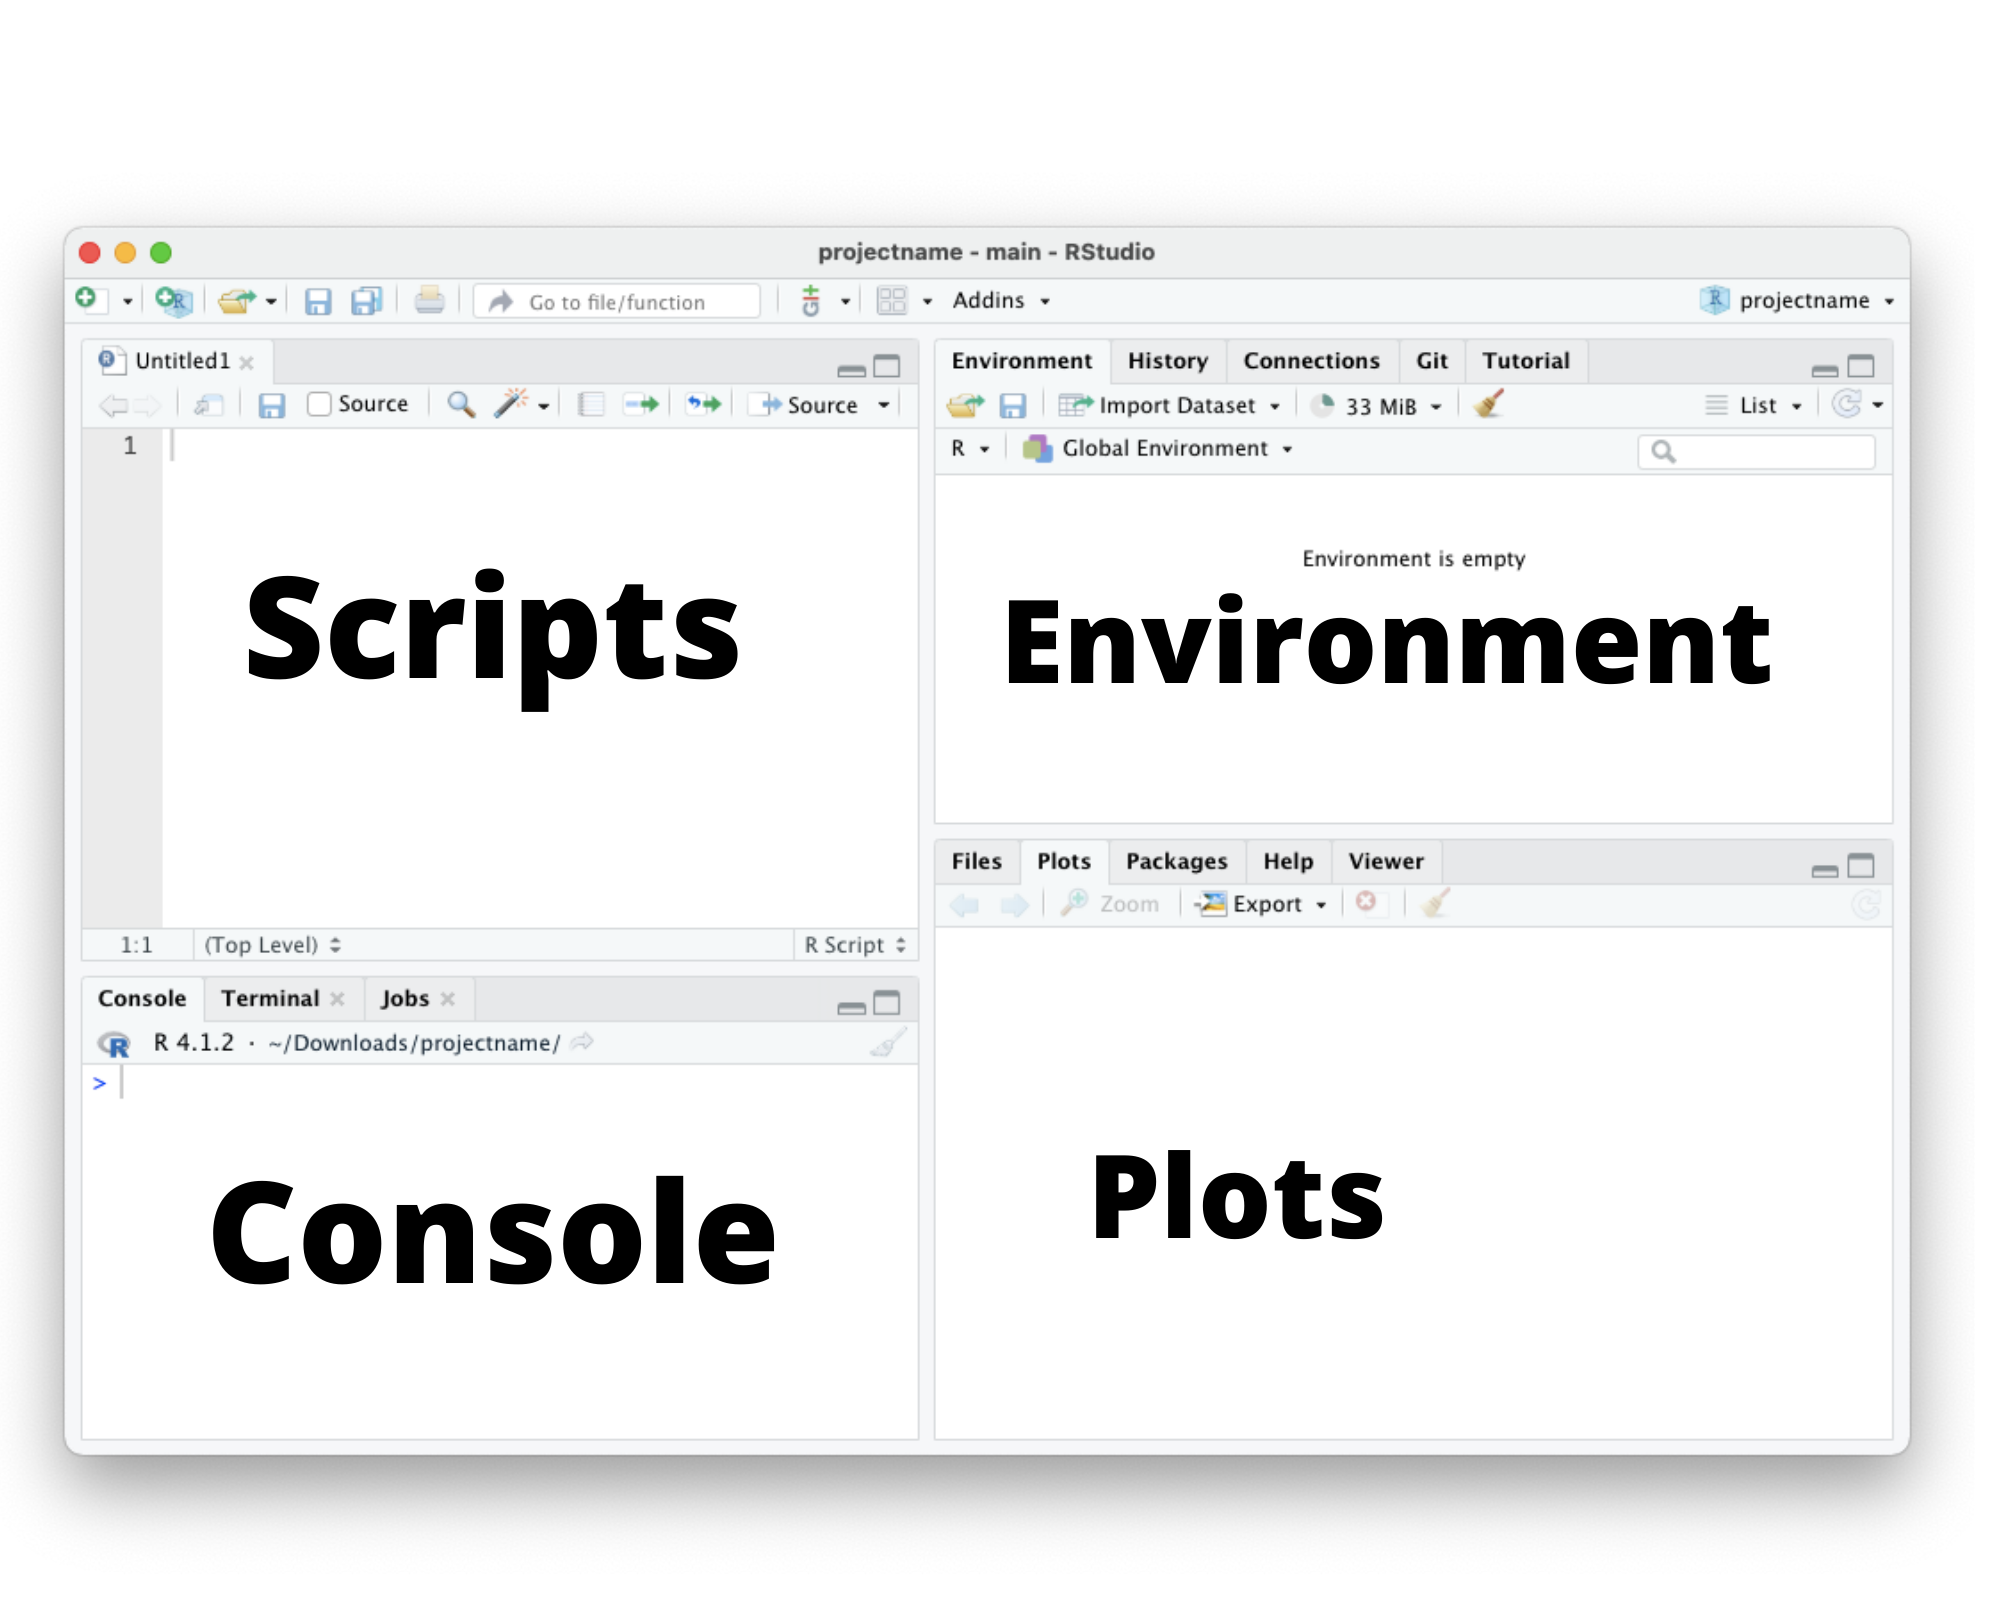
\includegraphics[width=3.125in,height=\textheight]{Console.png}\\
L'interface RStudio se présente ainsi par défaut. Nous pouvons voir une console, un environnement de travail, une partie pour les scripts et une autre pour la visualisation des graphiques.

\begin{itemize}
\tightlist
\item
  La \emph{console} peut servir à écrire une ligne d'instruction qui sera exécutée en appuyant sur Entrer.\\
\item
  La partie dédiée au \emph{scripts} permet d'écrire un ensemble de lignes de codes qui peuvent être exécutées par ordre voulu par l'utilisateur. En plus des scripts, on peut y visualiser nos tableaux de données qui sont décrits dans la section \ref{dataframe}.\\
\item
  Les graphes peuvent être visibles dans la partie \emph{Plots} de notre interface. Cette partie est un panneau contenant les onglets \emph{Viewer} pour les pages html, \emph{Files} pour naviguer dans les fichiers, \emph{Packages} pour gérer les packages installes et \emph{Help} pour chercher de l'aide.\\
\item
  La dernière partie c'est à dire \emph{Environment} est consacrée à la gestion de l'environnement de travail. Elle permet de voir les variable créé lors de notre session mais aussi d'avoir une idée sur leur structure
\end{itemize}

\hypertarget{firstcode}{%
\section{Premiers codes}\label{firstcode}}

Et si on écrivait notre premier code ?
Dans la section précédente nous avons présenté brièvement l'interface de RStudio, place maintenant à notre première instruction. Commencez par effectuer une petite opération d'addition (\texttt{2+3}) sur votre console puis appuyez sur Entrer.

\begin{Shaded}
\begin{Highlighting}[]
\DecValTok{2}\SpecialCharTok{+}\DecValTok{3}
\CommentTok{\#\textgreater{} [1] 5}
\end{Highlighting}
\end{Shaded}

Le résultat obtenu est tout naturellement \texttt{5}. Vous constatez que \texttt{{[}1{]}} précède le résultat de l'opération, en effet l'affichage se fait par défaut sous forme d'une liste\ref{list}.\\
La console peut être utilisée comme une calculatrice et supporte toute les opération arithmétique telle que la soustraction(\texttt{-}), l'addition(\texttt{+}), la multiplication(\texttt{*}), la division décimale(\texttt{/}), la division entière(\texttt{\%/\%}), le modulo\footnote{modulo : Cet opérateur renvoi le reste de la division entre deux nombres} (\texttt{\%\%}).\\
Le symbole (\texttt{\#}) sert à écrire une ligne de commentaire.

\begin{Shaded}
\begin{Highlighting}[]
\DecValTok{1}\SpecialCharTok{+}\DecValTok{2} \CommentTok{\#addition}

\DecValTok{1{-}2} \CommentTok{\#Soustraction}

\DecValTok{1}\SpecialCharTok{/}\DecValTok{2} \CommentTok{\#Division decimale}

\DecValTok{1}\SpecialCharTok{\%/\%}\DecValTok{2} \CommentTok{\#Division entiere}

\DecValTok{1}\SpecialCharTok{\%\%}\DecValTok{2} \CommentTok{\#Modulo}
\end{Highlighting}
\end{Shaded}

On peut aussi effectuer des assignations sans déclarer les variables au préalable comme l'indique le code suivant.

\begin{Shaded}
\begin{Highlighting}[]
\NormalTok{x }\OtherTok{=} \DecValTok{1} \CommentTok{\#affection de la valeur 1 à x}
\NormalTok{y }\OtherTok{\textless{}{-}} \DecValTok{2} \CommentTok{\#affection de la valeur 2 à y}
\NormalTok{x}\SpecialCharTok{+}\NormalTok{y }\CommentTok{\#somme de x et y (1+2)}
\CommentTok{\#\textgreater{} [1] 3}
\end{Highlighting}
\end{Shaded}

\hypertarget{data-R}{%
\section{Données sur R}\label{data-R}}

Il existe 6 principaux types simples de données sur R sont : \emph{logical}, \emph{integer}, \emph{double}, \emph{complex}, \emph{character}, \emph{raw}.\\
Il arrive qu'une structure de données se compose de types simples données, c'est ce que nous allons étudier dans cette section.

\hypertarget{vecteur}{%
\subsection{Vecteur}\label{vecteur}}

\hypertarget{duxe9finition}{%
\subsubsection*{Définition}\label{duxe9finition}}
\addcontentsline{toc}{subsubsection}{Définition}

Le vecteur est un objet de base de R qui correspond à une liste d'éléments. Ses propriétés fondamentales sont :

\begin{itemize}
\tightlist
\item
  Dimension unitaire (les vecteurs sont unidimensionnel)\\
\item
  Éléments de même type (Toutes les valeurs contenues dans un vecteur sont de même type)\\
\item
  Longueure égale au nombre d'éléments
\end{itemize}

\hypertarget{cruxe9ation}{%
\subsubsection*{Création}\label{cruxe9ation}}
\addcontentsline{toc}{subsubsection}{Création}

La fonction la plus classique pour créer un vecteur est \texttt{c(...)}. Elle prend comme argument les éléments du vecteur. Dans le code suivant, nous allons créer un vecteur contenant les valeurs de 1 jusqu'à 5 puis nous allons le nommer \texttt{myvector}

\begin{Shaded}
\begin{Highlighting}[]
\NormalTok{myvector }\OtherTok{\textless{}{-}} \FunctionTok{c}\NormalTok{(}\DecValTok{1}\NormalTok{,}\DecValTok{2}\NormalTok{,}\DecValTok{3}\NormalTok{,}\DecValTok{4}\NormalTok{,}\DecValTok{5}\NormalTok{) }\CommentTok{\#Création}
\NormalTok{myvector }\CommentTok{\#Affichage}
\CommentTok{\#\textgreater{} [1] 1 2 3 4 5}
\end{Highlighting}
\end{Shaded}

Maintenant que nous avons un vecteur, il est naturel de se demander comment accéder aux éléments de ce dernier. Facile ! Il suffit de mettre entre crochet (\texttt{{[}{]}}), juste après le nom de votre vecteur, l'indice de l'élément voulu sachant que sur R le comptage commence par 1 au lieu de 0. Par exemple, dans la cellule suivante, le code permet d'afficher le quatrième élément c'est-à-dire celui qui a pour indice 4 de \texttt{myvector}.

\begin{Shaded}
\begin{Highlighting}[]
\NormalTok{myvector[}\DecValTok{4}\NormalTok{]}
\CommentTok{\#\textgreater{} [1] 4}
\end{Highlighting}
\end{Shaded}

Vous pouvez aussi supprimer un élément d'un vecteur en essayant de l'afficher avec l'opposé de son indice. Supprimons le premier élément de \texttt{myvector} !

\begin{Shaded}
\begin{Highlighting}[]
\NormalTok{myvector[}\SpecialCharTok{{-}}\DecValTok{1}\NormalTok{]}
\CommentTok{\#\textgreater{} [1] 2 3 4 5}
\end{Highlighting}
\end{Shaded}

Il se peut qu'on veuille créer une séquence de valeurs avec un pas spécifié. Un exemple concret c'est de vouloir créer un vecteur nommé \texttt{evenVector} contenant tous les nombres pairs compris entre 0 et 100. L'utilisation de la fonction \texttt{c()} rendrait le travail fastidieux. La fonction \texttt{seq()} est plus adaptée à notre situation. Elle prend comme argument fom(le début de la séquence), to(la fin de la séquence), by(le pas de la séquence), etc. Pour en savoir plus vous pouvez exécuter la commande \texttt{?seq()}.

\begin{Shaded}
\begin{Highlighting}[]
\NormalTok{evenVector }\OtherTok{\textless{}{-}} \FunctionTok{seq}\NormalTok{(}\AttributeTok{from =} \DecValTok{0}\NormalTok{, }\AttributeTok{to =} \DecValTok{100}\NormalTok{, }\AttributeTok{by =} \DecValTok{2}\NormalTok{) }\CommentTok{\#Création }
\NormalTok{evenVector }\CommentTok{\#Affichage}
\CommentTok{\#\textgreater{}  [1]   0   2   4   6   8  10  12  14  16  18  20  22  24  26}
\CommentTok{\#\textgreater{} [15]  28  30  32  34  36  38  40  42  44  46  48  50  52  54}
\CommentTok{\#\textgreater{} [29]  56  58  60  62  64  66  68  70  72  74  76  78  80  82}
\CommentTok{\#\textgreater{} [43]  84  86  88  90  92  94  96  98 100}
\end{Highlighting}
\end{Shaded}

Si le pas de la séquence est de 1, on peut utiliser à la place de \texttt{seq()} l'opérateur \texttt{:} de premier terme le début de la séquence et de second terme la fin de la séquence. L'exemple qui suit permet de créer le vecteur \texttt{myvector} contenant tous les entiers de 1 à 5.

\begin{Shaded}
\begin{Highlighting}[]
\NormalTok{myvector }\OtherTok{\textless{}{-}} \DecValTok{1}\SpecialCharTok{:}\DecValTok{5}
\NormalTok{myvector}
\CommentTok{\#\textgreater{} [1] 1 2 3 4 5}
\end{Highlighting}
\end{Shaded}

Il est possible de créer un vecteur d'éléments répétitifs avec la fonction \texttt{rep()}. Supposons que nous voulons créer le vecteur \texttt{repvector} contenant 5 fois de suite tous les entiers de 1 à 10, nous allons donner en premier argument à la fonction \texttt{rep()} l'objet à répéter (\texttt{1:10}) et comme second argument le nombre de répétitions(\texttt{5}).

\begin{Shaded}
\begin{Highlighting}[]
\NormalTok{repvector }\OtherTok{\textless{}{-}} \FunctionTok{rep}\NormalTok{(}\DecValTok{1}\SpecialCharTok{:}\DecValTok{10}\NormalTok{,}\DecValTok{5}\NormalTok{)}
\NormalTok{repvector}
\CommentTok{\#\textgreater{}  [1]  1  2  3  4  5  6  7  8  9 10  1  2  3  4  5  6  7  8}
\CommentTok{\#\textgreater{} [19]  9 10  1  2  3  4  5  6  7  8  9 10  1  2  3  4  5  6}
\CommentTok{\#\textgreater{} [37]  7  8  9 10  1  2  3  4  5  6  7  8  9 10}
\end{Highlighting}
\end{Shaded}

\hypertarget{facteur}{%
\subsection{Facteur}\label{facteur}}

\hypertarget{duxe9finition-1}{%
\subsubsection*{Définition}\label{duxe9finition-1}}
\addcontentsline{toc}{subsubsection}{Définition}

Le facteur (\emph{factor}) est un vecteur de valeurs d'une variable catégorielle. Très souvevent, les variables qualitatives sont catégorielles c'est le cas du sexe(Homme, Femme), des questions directes(Oui, Non), etc.C'est d'ailleurs la raison de l'existance de cet objet sur R qui est très utiles dans certaines representations graphiques.Le caractère principal de \emph{factor} est qu'il dispose de niveaux appelés \texttt{levels}. Ces derniers sont uniques et peuvent avoir des valeurs qui ne sont pas contenus par le facteur.

\hypertarget{cruxe9ation-1}{%
\subsubsection*{Création}\label{cruxe9ation-1}}
\addcontentsline{toc}{subsubsection}{Création}

Pour créer un facteur, on commence par créer un vecteur puis avec la fonction \texttt{factor()} nous pouvons le transformer en objet de type facteur. Par défaut, les niveaux des facteurs sont les modalités prises par le vecteur. Pour modifier les niveaux on utilise l'argument \texttt{levels} de la fonction \texttt{factor()} pour spécifier notre vecteur de niveaux.
On se propose de transformer en facteur le vecteur \texttt{animal} de modalités \emph{chat}, \emph{souris}, \emph{chien} en un facteur de niveaux \emph{chat}, \emph{souris}, \emph{chien} et \emph{rat}.

\begin{Shaded}
\begin{Highlighting}[]
\NormalTok{animal }\OtherTok{\textless{}{-}} \FunctionTok{c}\NormalTok{(}\StringTok{"souris"}\NormalTok{,}\StringTok{"souris"}\NormalTok{,}\StringTok{"chien"}\NormalTok{,}\StringTok{"chat"}\NormalTok{,}\StringTok{"chien"}\NormalTok{,}\StringTok{"chat"}\NormalTok{,}\StringTok{"souris"}\NormalTok{,}\StringTok{"chat"}\NormalTok{,}\StringTok{"chat"}\NormalTok{,}\StringTok{"chien"}\NormalTok{)}
\NormalTok{myfactor }\OtherTok{\textless{}{-}} \FunctionTok{factor}\NormalTok{(animal,}\AttributeTok{levels =} \FunctionTok{c}\NormalTok{(}\StringTok{\textquotesingle{}chat\textquotesingle{}}\NormalTok{,}\StringTok{\textquotesingle{}souris\textquotesingle{}}\NormalTok{,}\StringTok{\textquotesingle{}chien\textquotesingle{}}\NormalTok{,}\StringTok{\textquotesingle{}rat\textquotesingle{}}\NormalTok{))}
\NormalTok{myfactor}
\CommentTok{\#\textgreater{}  [1] souris souris chien  chat   chien  chat   souris chat  }
\CommentTok{\#\textgreater{}  [9] chat   chien }
\CommentTok{\#\textgreater{} Levels: chat souris chien rat}
\end{Highlighting}
\end{Shaded}

\hypertarget{list}{%
\subsection{Liste}\label{list}}

\hypertarget{duxe9finition-2}{%
\subsubsection*{Définition}\label{duxe9finition-2}}
\addcontentsline{toc}{subsubsection}{Définition}

Une liste est un objet pouvant contenir des éléments de tous types. L'homogénéité du type des éléments n'est pas obligatoire dans une liste c'est à dire qu'elle peut contenir des listes, des vecteurs, des matrices, des fonctions etc. On peut nommer les éléments d'une liste lors de sa création en effectuant des affections.

\hypertarget{cruxe9ation-2}{%
\subsubsection*{Création}\label{cruxe9ation-2}}
\addcontentsline{toc}{subsubsection}{Création}

La création d'une liste se fait avec la fonction \texttt{list()} qui prend en argument les éléments à concaténer.

\begin{Shaded}
\begin{Highlighting}[]
\NormalTok{mylist }\OtherTok{=} \FunctionTok{list}\NormalTok{(}\AttributeTok{num =} \FunctionTok{c}\NormalTok{(}\DecValTok{1}\NormalTok{,}\DecValTok{2}\NormalTok{,}\DecValTok{3}\NormalTok{), }\AttributeTok{char =} \StringTok{\textquotesingle{}character\textquotesingle{}}\NormalTok{)}
\NormalTok{mylist}
\CommentTok{\#\textgreater{} $num}
\CommentTok{\#\textgreater{} [1] 1 2 3}
\CommentTok{\#\textgreater{} }
\CommentTok{\#\textgreater{} $char}
\CommentTok{\#\textgreater{} [1] "character"}
\end{Highlighting}
\end{Shaded}

On peut accéder à un élément par son nom en utilisant le symbole \texttt{\$} (\texttt{malist\$nomElement}). L'accès à l'élément \texttt{num} de \texttt{mylist} peut se faire de la manière suivante :

\begin{Shaded}
\begin{Highlighting}[]
\NormalTok{mylist}\SpecialCharTok{$}\NormalTok{num}
\CommentTok{\#\textgreater{} [1] 1 2 3}
\end{Highlighting}
\end{Shaded}

Un autre moyen d'accéder à un élément d'une liste c'est par son indice mis entre deux crochets (\texttt{{[}{[}index{]}{]}}) juste après le nom de la liste. On peut reprendre l'accès à l'élément \texttt{num} par indexation.

\begin{Shaded}
\begin{Highlighting}[]
\NormalTok{mylist[[}\DecValTok{1}\NormalTok{]]}
\CommentTok{\#\textgreater{} [1] 1 2 3}
\end{Highlighting}
\end{Shaded}

On peut modifier l'élément \texttt{num} de mylist en lui affectant une nouvelle valeur.

\begin{Shaded}
\begin{Highlighting}[]
\NormalTok{mylist}\SpecialCharTok{$}\NormalTok{num }\OtherTok{=} \DecValTok{1}\SpecialCharTok{:}\DecValTok{10}
\NormalTok{mylist}\SpecialCharTok{$}\NormalTok{num}
\CommentTok{\#\textgreater{}  [1]  1  2  3  4  5  6  7  8  9 10}
\end{Highlighting}
\end{Shaded}

L'ajout d'un nouvel élément dans \texttt{mylist} peut aussi se faire facilement. Si on se propose d'ajouter un élément nommé \texttt{logical} qui reçoit initialement \texttt{TRUE} on peut procéder ainsi :

\begin{Shaded}
\begin{Highlighting}[]
\NormalTok{mylist}\SpecialCharTok{$}\NormalTok{logical }\OtherTok{=} \ConstantTok{TRUE}
\NormalTok{mylist}
\CommentTok{\#\textgreater{} $num}
\CommentTok{\#\textgreater{}  [1]  1  2  3  4  5  6  7  8  9 10}
\CommentTok{\#\textgreater{} }
\CommentTok{\#\textgreater{} $char}
\CommentTok{\#\textgreater{} [1] "character"}
\CommentTok{\#\textgreater{} }
\CommentTok{\#\textgreater{} $logical}
\CommentTok{\#\textgreater{} [1] TRUE}
\end{Highlighting}
\end{Shaded}

\hypertarget{matrice}{%
\subsection{Matrice}\label{matrice}}

\hypertarget{duxe9finition-3}{%
\subsubsection*{Définition}\label{duxe9finition-3}}
\addcontentsline{toc}{subsubsection}{Définition}

Un matrice est un un tableau dont les colonnes sont des vecteurs de même type et de même taille. Autrement dit, la matrice est un objet de deux dimensions dont tous les éléments sont de type homogène. R ne considère pas un vecteur comme une matrice colonne ou ligne, ce sont deux types de structures différentes.

\hypertarget{cruxe9ation-3}{%
\subsubsection*{Création}\label{cruxe9ation-3}}
\addcontentsline{toc}{subsubsection}{Création}

Une matrice colonne se crée avec la fonction \texttt{cbind()} et la matrice ligne par \texttt{rbind()}. Pour créer une matrice de plusieurs colonnes on utilise la fonction \texttt{matrix()}.
Vous pouvez avoir une documentation complète de ces fonctions en exécutant la commande faisant précéder d'un point d'interrogation le nom de votre fonction ( \emph{Exemple} : \texttt{?cbind()}) dans votre console.

\begin{Shaded}
\begin{Highlighting}[]
\CommentTok{\#matrice colonne}
\NormalTok{colMatrix }\OtherTok{\textless{}{-}} \FunctionTok{cbind}\NormalTok{(}\DecValTok{1}\SpecialCharTok{:}\DecValTok{5}\NormalTok{)}
\NormalTok{colMatrix}
\CommentTok{\#\textgreater{}      [,1]}
\CommentTok{\#\textgreater{} [1,]    1}
\CommentTok{\#\textgreater{} [2,]    2}
\CommentTok{\#\textgreater{} [3,]    3}
\CommentTok{\#\textgreater{} [4,]    4}
\CommentTok{\#\textgreater{} [5,]    5}
\end{Highlighting}
\end{Shaded}

\begin{Shaded}
\begin{Highlighting}[]
\CommentTok{\#matrice ligne}
\NormalTok{rowMatrix }\OtherTok{\textless{}{-}} \FunctionTok{rbind}\NormalTok{(}\DecValTok{1}\SpecialCharTok{:}\DecValTok{5}\NormalTok{)}
\NormalTok{rowMatrix}
\CommentTok{\#\textgreater{}      [,1] [,2] [,3] [,4] [,5]}
\CommentTok{\#\textgreater{} [1,]    1    2    3    4    5}
\end{Highlighting}
\end{Shaded}

\begin{Shaded}
\begin{Highlighting}[]
\CommentTok{\#matrice}
\NormalTok{Matrix }\OtherTok{\textless{}{-}} \FunctionTok{matrix}\NormalTok{(}\FunctionTok{c}\NormalTok{(}\AttributeTok{x=}\NormalTok{ (}\DecValTok{1}\SpecialCharTok{:}\DecValTok{5}\NormalTok{), }\AttributeTok{y =} \FunctionTok{rep}\NormalTok{(}\DecValTok{1}\NormalTok{,}\DecValTok{5}\NormalTok{)),}\AttributeTok{nrow =} \DecValTok{5}\NormalTok{)}
\NormalTok{Matrix}
\CommentTok{\#\textgreater{}      [,1] [,2]}
\CommentTok{\#\textgreater{} [1,]    1    1}
\CommentTok{\#\textgreater{} [2,]    2    1}
\CommentTok{\#\textgreater{} [3,]    3    1}
\CommentTok{\#\textgreater{} [4,]    4    1}
\CommentTok{\#\textgreater{} [5,]    5    1}
\end{Highlighting}
\end{Shaded}

On peut accéder aux éléments de la matrice par leurs indices. Comme on le fait en maths, il faut d'abord mettre le numéro de la ligne puis le numéro de la colonne séparée par une virgule.
On peut afficher une ligne (respectivement une colonne )toute entière en spécifiant seulement l'indice de la ligne (respectivement la colonne).

\begin{Shaded}
\begin{Highlighting}[]
\CommentTok{\# Accès à l\textquotesingle{}élément de la ligne 4 et de la colonne 1}
\NormalTok{Matrix[}\DecValTok{4}\NormalTok{,}\DecValTok{1}\NormalTok{]}
\CommentTok{\#\textgreater{} [1] 4}
\end{Highlighting}
\end{Shaded}

\begin{Shaded}
\begin{Highlighting}[]
\CommentTok{\# Accès à  la ligne 2 }
\NormalTok{Matrix[}\DecValTok{2}\NormalTok{,]}
\CommentTok{\#\textgreater{} [1] 2 1}
\end{Highlighting}
\end{Shaded}

\begin{Shaded}
\begin{Highlighting}[]
\CommentTok{\# Accès à la colonne 3}
\NormalTok{Matrix[,}\DecValTok{2}\NormalTok{]}
\CommentTok{\#\textgreater{} [1] 1 1 1 1 1}
\end{Highlighting}
\end{Shaded}

\hypertarget{dataframe}{%
\subsection{Tableau de données ou Data frame}\label{dataframe}}

\hypertarget{duxe9finition-4}{%
\subsubsection*{Définition}\label{duxe9finition-4}}
\addcontentsline{toc}{subsubsection}{Définition}

Un tableau de données (data frame) est comme la matrice, un objet de deux dimensions sauf qu'il peut contenir des colonnes de types différents. Chaque colonne doit contenir des éléments de même type. La data.frame est un objet très utilisé sur R et ce sera le cas dans les chapitres suivants de ce livre.

\hypertarget{cruxe9ation-4}{%
\subsubsection*{Création}\label{cruxe9ation-4}}
\addcontentsline{toc}{subsubsection}{Création}

La fonction \texttt{data.frame()} permet de créer un un tableau de données. Elle prend en argument des vecteurs de même longueur. Il en existe d'autres arguments pour cette fonction, pour en savoir plus vous pouvez exécuter \texttt{?data.frame()}.

\begin{Shaded}
\begin{Highlighting}[]
\NormalTok{x }\OtherTok{=} \FunctionTok{c}\NormalTok{(}\DecValTok{12}\NormalTok{,}\DecValTok{67}\NormalTok{,}\DecValTok{13}\NormalTok{)}
\NormalTok{y }\OtherTok{=} \FunctionTok{c}\NormalTok{(}\StringTok{\textquotesingle{}A\textquotesingle{}}\NormalTok{,}\StringTok{\textquotesingle{}B\textquotesingle{}}\NormalTok{,}\StringTok{\textquotesingle{}C\textquotesingle{}}\NormalTok{)}
\NormalTok{tableau }\OtherTok{=} \FunctionTok{data.frame}\NormalTok{(x,y)}
\NormalTok{tableau}
\CommentTok{\#\textgreater{}    x y}
\CommentTok{\#\textgreater{} 1 12 A}
\CommentTok{\#\textgreater{} 2 67 B}
\CommentTok{\#\textgreater{} 3 13 C}
\end{Highlighting}
\end{Shaded}

L'accès à un élément peut se faire de la même manière qu'avec les matrices. Pour accéder à une colonne par son nom on utilise le symbole \texttt{\$} comme dans la section liste. Les codes suivants permettent d'accéder à l'élément ``B'' de \texttt{tableau} de plusieurs façons.

\begin{Shaded}
\begin{Highlighting}[]
\CommentTok{\#Indexiation}
\NormalTok{tableau[}\DecValTok{2}\NormalTok{,}\DecValTok{2}\NormalTok{]}
\CommentTok{\#\textgreater{} [1] "B"}
\end{Highlighting}
\end{Shaded}

\begin{Shaded}
\begin{Highlighting}[]
\CommentTok{\#Par le nom de la colonne}
\NormalTok{tableau}\SpecialCharTok{$}\NormalTok{y[}\DecValTok{2}\NormalTok{]}
\CommentTok{\#\textgreater{} [1] "B"}
\end{Highlighting}
\end{Shaded}

\begin{Shaded}
\begin{Highlighting}[]
\NormalTok{tableau[[}\StringTok{\textquotesingle{}y\textquotesingle{}}\NormalTok{]][}\DecValTok{2}\NormalTok{]}
\CommentTok{\#\textgreater{} [1] "B"}
\end{Highlighting}
\end{Shaded}

\hypertarget{les-boucles-et-conditions}{%
\section{Les boucles et conditions}\label{les-boucles-et-conditions}}

\hypertarget{les-boucles}{%
\subsection{Les boucles}\label{les-boucles}}

Les boucles permettent de gérer des instructions répétitives. Sur R il est plus pratique d'utiliser la vectorisation, mais pour débuter, les boucles feront l'affaire.

\hypertarget{for}{%
\subsubsection*{for}\label{for}}
\addcontentsline{toc}{subsubsection}{for}

La boucle for permet d'itérer sur un vecteur de longueur connu d'avance. La syntaxe est la suivante :

\begin{Shaded}
\begin{Highlighting}[]
\ControlFlowTok{for}\NormalTok{ (variable }\ControlFlowTok{in}\NormalTok{ vector) \{}
\NormalTok{  statements}
\NormalTok{\}}
\end{Highlighting}
\end{Shaded}

Un exemple de création d'un vecteur de 5 éléments contenant les carré des nombre compris entre 1 et 5

\begin{Shaded}
\begin{Highlighting}[]
\CommentTok{\#Initialisation}
\NormalTok{carrevector }\OtherTok{=} \DecValTok{0}
\CommentTok{\#Boucle}
\ControlFlowTok{for}\NormalTok{ (i }\ControlFlowTok{in} \DecValTok{1}\SpecialCharTok{:}\DecValTok{5}\NormalTok{) \{}
\NormalTok{  carrevector[i]}\OtherTok{=}\NormalTok{i}\SpecialCharTok{\^{}}\DecValTok{2}
\NormalTok{\}}
\CommentTok{\#affichage}
\NormalTok{carrevector}
\CommentTok{\#\textgreater{} [1]  1  4  9 16 25}
\end{Highlighting}
\end{Shaded}

\hypertarget{while}{%
\subsubsection*{While}\label{while}}
\addcontentsline{toc}{subsubsection}{While}

Si le nombre d'itérations n'est pas connu d'avance alors que la condition d'arrêt si, il est préférable d'utiliser la boucle while. Elle permet de répéter une instruction tant qu'une condition est satisfaite. la syntaxe est la suivante :

\begin{Shaded}
\begin{Highlighting}[]
\ControlFlowTok{while}\NormalTok{ (condition) \{}
\NormalTok{  statements}
\NormalTok{\}}
\end{Highlighting}
\end{Shaded}

Avec la boucle while on peut chercher le premier élément supérieur à 10 dans \texttt{carrevector}. Les deux conditions d'arrêts sont alors : l'élément(\texttt{x}) supérieur à 10 et(\texttt{\&}) l'indice(\texttt{j}) supérieur à la longueur du vecteur(\texttt{5}).

\begin{Shaded}
\begin{Highlighting}[]
\CommentTok{\# Initialisation}
\NormalTok{j }\OtherTok{=} \DecValTok{1}
\CommentTok{\# Boucle}
\ControlFlowTok{while}\NormalTok{ (carrevector[j]}\SpecialCharTok{\textless{}=}\DecValTok{10} \SpecialCharTok{\&}\NormalTok{ j}\SpecialCharTok{\textless{}=} \DecValTok{5}\NormalTok{)\{}
\NormalTok{  j}\OtherTok{=}\NormalTok{j}\SpecialCharTok{+}\DecValTok{1}
\NormalTok{\}}
\NormalTok{x}\OtherTok{=}\NormalTok{carrevector[j]}
\CommentTok{\# Affichage}
\NormalTok{x}
\CommentTok{\#\textgreater{} [1] 16}
\end{Highlighting}
\end{Shaded}

\hypertarget{les-conditions}{%
\subsection{Les conditions}\label{les-conditions}}

Elles permettent d'exécuter des instructions si une ou des conditions sont satisfaites. la syntaxe la plus simple est :

\begin{Shaded}
\begin{Highlighting}[]
\ControlFlowTok{if}\NormalTok{ (condition) \{}
  \CommentTok{\#statements}
\NormalTok{\}}\ControlFlowTok{else}\NormalTok{\{}
  \CommentTok{\#statements}
\NormalTok{\}}
\end{Highlighting}
\end{Shaded}

\textbf{Exemple} :

\begin{Shaded}
\begin{Highlighting}[]
\NormalTok{num }\OtherTok{=} \DecValTok{10}
\ControlFlowTok{if}\NormalTok{ (num }\SpecialCharTok{\textgreater{}} \DecValTok{0}\NormalTok{) \{}
  \FunctionTok{print}\NormalTok{(}\StringTok{\textquotesingle{}Ce nombre est positif\textquotesingle{}}\NormalTok{)}
\NormalTok{\}}\ControlFlowTok{else}\NormalTok{\{}
  \FunctionTok{print}\NormalTok{(}\StringTok{\textquotesingle{}Ce nombre est negatif\textquotesingle{}}\NormalTok{)}
\NormalTok{\}}
\CommentTok{\#\textgreater{} [1] "Ce nombre est positif"}
\end{Highlighting}
\end{Shaded}

\hypertarget{les-fonctions}{%
\section{Les fonctions}\label{les-fonctions}}

Si dans un projet vous aurez à utiliser plusieurs fois un bloc d'instructions, l'idéal c'est de créer des fonctions. Pour cela, on a besoin de \texttt{function()} que l'on assigne au nom de notre fonction.
Les fonctions peuvent retourner une valeur ou bien exécuter seulement un ensemble d'instructions.

\begin{Shaded}
\begin{Highlighting}[]
\NormalTok{mafonction }\OtherTok{=}\NormalTok{ name }\OtherTok{\textless{}{-}} \ControlFlowTok{function}\NormalTok{(arguments) \{}
\NormalTok{  instructions}
  \FunctionTok{return}\NormalTok{(valuer)}
\NormalTok{\}}
\end{Highlighting}
\end{Shaded}

Pour créer la fonction \texttt{addition} qui somme deux éléments \texttt{x} et \texttt{y} on procède ainsi :

\begin{Shaded}
\begin{Highlighting}[]
\NormalTok{addition }\OtherTok{\textless{}{-}} \ControlFlowTok{function}\NormalTok{(x,y)\{}
  \FunctionTok{return}\NormalTok{(x}\SpecialCharTok{+}\NormalTok{y)}
\NormalTok{\}}
\CommentTok{\#Ou bien}
\NormalTok{addition }\OtherTok{\textless{}{-}} \ControlFlowTok{function}\NormalTok{(x,y)\{}
\NormalTok{  x}\SpecialCharTok{+}\NormalTok{y}
\NormalTok{\}}
\end{Highlighting}
\end{Shaded}

Pour utiliser la fonction il suffit de l'appeler en indiquant les valeurs de ses arguments entre parenthèses.

\begin{Shaded}
\begin{Highlighting}[]
\CommentTok{\# somme de 10 et de 4}
\FunctionTok{addition}\NormalTok{(}\DecValTok{10}\NormalTok{,}\DecValTok{4}\NormalTok{)}
\CommentTok{\#\textgreater{} [1] 14}
\end{Highlighting}
\end{Shaded}

\hypertarget{liens-utils}{%
\section*{Liens utils}\label{liens-utils}}
\addcontentsline{toc}{section}{Liens utils}

\citet{base}\strut \\
\url{https://cran.r-project.org/doc/contrib/Paradis-rdebuts_fr.pdf}

\hypertarget{part-ii-regressions}{%
\part{II-Regressions}\label{part-ii-regressions}}

\hypertarget{simple-lm}{%
\chapter{La régression linéaire simple}\label{simple-lm}}

You can add parts to organize one or more book chapters together. Parts can be inserted at the top of an .Rmd file, before the first-level chapter heading in that same file.

Add a numbered part: \texttt{\#\ (PART)\ Act\ one\ \{-\}} (followed by \texttt{\#\ A\ chapter})

Add an unnumbered part: \texttt{\#\ (PART\textbackslash{}*)\ Act\ one\ \{-\}} (followed by \texttt{\#\ A\ chapter})

Add an appendix as a special kind of un-numbered part: \texttt{\#\ (APPENDIX)\ Other\ stuff\ \{-\}} (followed by \texttt{\#\ A\ chapter}). Chapters in an appendix are prepended with letters instead of numbers.

\hypertarget{multiple-lm}{%
\chapter{La régression linéaire multiple}\label{multiple-lm}}

\hypertarget{footnotes}{%
\section{Footnotes}\label{footnotes}}

Footnotes are put inside the square brackets after a caret \texttt{\^{}{[}{]}}. Like this one \footnote{This is a footnote.}.

\hypertarget{citations}{%
\section{Citations}\label{citations}}

Reference items in your bibliography file(s) using \texttt{@key}.

For example, we are using the \textbf{bookdown} package \citep{R-bookdown} (check out the last code chunk in index.Rmd to see how this citation key was added) in this sample book, which was built on top of R Markdown and \textbf{knitr} \citep{xie2015} (this citation was added manually in an external file book.bib).
Note that the \texttt{.bib} files need to be listed in the index.Rmd with the YAML \texttt{bibliography} key.

The \texttt{bs4\_book} theme makes footnotes appear inline when you click on them. In this example book, we added \texttt{csl:\ chicago-fullnote-bibliography.csl} to the \texttt{index.Rmd} YAML, and include the \texttt{.csl} file. To download a new style, we recommend: \url{https://www.zotero.org/styles/}

The RStudio Visual Markdown Editor can also make it easier to insert citations: \url{https://rstudio.github.io/visual-markdown-editing/\#/citations}

\hypertarget{glm}{%
\chapter{Le modèle linéaire généralisé}\label{glm}}

\hypertarget{equations}{%
\section{Equations}\label{equations}}

Here is an equation.

\begin{equation} 
  f\left(k\right) = \binom{n}{k} p^k\left(1-p\right)^{n-k}
  \label{eq:binom}
\end{equation}

You may refer to using \texttt{\textbackslash{}@ref(eq:binom)}, like see Equation \eqref{eq:binom}.

\hypertarget{theorems-and-proofs}{%
\section{Theorems and proofs}\label{theorems-and-proofs}}

Labeled theorems can be referenced in text using \texttt{\textbackslash{}@ref(thm:tri)}, for example, check out this smart theorem \ref{thm:tri}.

\begin{theorem}
\protect\hypertarget{thm:tri}{}\label{thm:tri}For a right triangle, if \(c\) denotes the \emph{length} of the hypotenuse
and \(a\) and \(b\) denote the lengths of the \textbf{other} two sides, we have
\[a^2 + b^2 = c^2\]
\end{theorem}

Read more here \url{https://bookdown.org/yihui/bookdown/markdown-extensions-by-bookdown.html}.

\hypertarget{callout-blocks}{%
\section{Callout blocks}\label{callout-blocks}}

The \texttt{bs4\_book} theme also includes special callout blocks, like this \texttt{.rmdnote}.

You can use \textbf{markdown} inside a block.

\begin{Shaded}
\begin{Highlighting}[]
\FunctionTok{head}\NormalTok{(beaver1, }\AttributeTok{n =} \DecValTok{5}\NormalTok{)}
\CommentTok{\#\textgreater{}   day time  temp activ}
\CommentTok{\#\textgreater{} 1 346  840 36.33     0}
\CommentTok{\#\textgreater{} 2 346  850 36.34     0}
\CommentTok{\#\textgreater{} 3 346  900 36.35     0}
\CommentTok{\#\textgreater{} 4 346  910 36.42     0}
\CommentTok{\#\textgreater{} 5 346  920 36.55     0}
\end{Highlighting}
\end{Shaded}

It is up to the user to define the appearance of these blocks for LaTeX output.

You may also use: \texttt{.rmdcaution}, \texttt{.rmdimportant}, \texttt{.rmdtip}, or \texttt{.rmdwarning} as the block name.

The R Markdown Cookbook provides more help on how to use custom blocks to design your own callouts: \url{https://bookdown.org/yihui/rmarkdown-cookbook/custom-blocks.html}

\hypertarget{anova1}{%
\chapter{Analyse de la variance à un facteur}\label{anova1}}

\hypertarget{publishing}{%
\section{Publishing}\label{publishing}}

HTML books can be published online, see: \url{https://bookdown.org/yihui/bookdown/publishing.html}

\hypertarget{pages}{%
\section{404 pages}\label{pages}}

By default, users will be directed to a 404 page if they try to access a webpage that cannot be found. If you'd like to customize your 404 page instead of using the default, you may add either a \texttt{\_404.Rmd} or \texttt{\_404.md} file to your project root and use code and/or Markdown syntax.

\hypertarget{metadata-for-sharing}{%
\section{Metadata for sharing}\label{metadata-for-sharing}}

Bookdown HTML books will provide HTML metadata for social sharing on platforms like Twitter, Facebook, and LinkedIn, using information you provide in the \texttt{index.Rmd} YAML. To setup, set the \texttt{url} for your book and the path to your \texttt{cover-image} file. Your book's \texttt{title} and \texttt{description} are also used.

This \texttt{bs4\_book} provides enhanced metadata for social sharing, so that each chapter shared will have a unique description, auto-generated based on the content.

Specify your book's source repository on GitHub as the \texttt{repo} in the \texttt{\_output.yml} file, which allows users to view each chapter's source file or suggest an edit. Read more about the features of this output format here:

\url{https://pkgs.rstudio.com/bookdown/reference/bs4_book.html}

Or use:

\begin{Shaded}
\begin{Highlighting}[]
\NormalTok{?bookdown}\SpecialCharTok{::}\NormalTok{bs4\_book}
\end{Highlighting}
\end{Shaded}

\hypertarget{anova2}{%
\chapter{Analyse de la variance à deux facteurs}\label{anova2}}

\hypertarget{ancova}{%
\chapter{Analyse de la covariance}\label{ancova}}

\hypertarget{part-iii-suxe9ries-chronologiques}{%
\part{III-Séries chronologiques}\label{part-iii-suxe9ries-chronologiques}}

\hypertarget{intro-ts}{%
\chapter{Introduction}\label{intro-ts}}

\hypertarget{duxe9finition-5}{%
\section{Définition}\label{duxe9finition-5}}

\hypertarget{exemples}{%
\section{Exemples}\label{exemples}}

\hypertarget{tendances-et-saisonnalituxe9s}{%
\chapter{Tendances et saisonnalités}\label{tendances-et-saisonnalituxe9s}}

\hypertarget{processus-stationnaire}{%
\section{Processus stationnaire}\label{processus-stationnaire}}

\hypertarget{estimation-paramuxe9trique-de-la-tendance}{%
\section{Estimation paramétrique de la tendance}\label{estimation-paramuxe9trique-de-la-tendance}}

\hypertarget{estimation-non-paramuxe9trique}{%
\section{Estimation non paramétrique}\label{estimation-non-paramuxe9trique}}

\hypertarget{elimination-du-trend-et-de-la-saisonnalituxe9}{%
\section{Elimination du trend et de la saisonnalité}\label{elimination-du-trend-et-de-la-saisonnalituxe9}}

\hypertarget{series-stat}{%
\chapter{Séries stationnaires}\label{series-stat}}

\hypertarget{processus-linuxe9aires-et-processus-linuxe9aires-guxe9nuxe9raux}{%
\section{Processus linéaires et processus linéaires généraux}\label{processus-linuxe9aires-et-processus-linuxe9aires-guxe9nuxe9raux}}

\hypertarget{les-processus-armapq}{%
\section{Les processus ARMA(p,q)}\label{les-processus-armapq}}

\hypertarget{processusmaq}{%
\subsection{ProcessusMA(q)}\label{processusmaq}}

\hypertarget{processus-arp}{%
\subsection{Processus AR(p)}\label{processus-arp}}

\hypertarget{autocovariance-des-processus-arma}{%
\section{Autocovariance des processus ARMA}\label{autocovariance-des-processus-arma}}

\hypertarget{proc-non-stat}{%
\chapter{Séries non stationnaires}\label{proc-non-stat}}

\hypertarget{processus-arima}{%
\section{Processus ARIMA}\label{processus-arima}}

\hypertarget{processus-sarima}{%
\section{Processus SARIMA}\label{processus-sarima}}

\hypertarget{ARCH-GARCH}{%
\chapter{Processus ARCH et GARCH}\label{ARCH-GARCH}}

\hypertarget{duxe9finition-6}{%
\section{Définition}\label{duxe9finition-6}}

\hypertarget{moduxe8les-arch}{%
\section{Modèles ARCH}\label{moduxe8les-arch}}

\hypertarget{moduxe8les-garch}{%
\section{Modèles GARCH}\label{moduxe8les-garch}}

\hypertarget{moduxe8lesarma-garch}{%
\section{ModèlesARMA-GARCH}\label{moduxe8lesarma-garch}}

  \bibliography{book.bib,packages.bib}

\end{document}
